\documentclass[compress]{beamer}        % [compress] (written before {beamer} <=> navigation bar one line, all subsections in 1 line instead of 2

% Setup appearance:
\usetheme{CambridgeUS}
%	AnnArbor | Antibes | Bergen |
%	Berkeley | Berlin | Boadilla |
%	boxes | CambridgeUS | Copenhagen |
%	Darmstadt | default | Dresden |
%	Frankfurt | Goettingen |Hannover |
%	Ilmenau | JuanLesPins | Luebeck |
%	Madrid | Malmoe | Marburg |
%	Montpellier | PaloAlto | Pittsburgh |
%	Rochester | Singapore | Szeged |
%	Warsaw
%

\useoutertheme[footline=authorinstitute,subsection=false]{miniframes}
\usecolortheme{whale}

%	albatross | beaver | beetle |
%	crane | default | dolphin |
%	dove | fly | lily | orchid |
%	rose |seagull | seahorse |
%	sidebartab | structure |
%	whale | wolverine


\setbeamertemplate{footline}
{
  \hbox{%
  \begin{beamercolorbox}[wd=.25\paperwidth,ht=2.25ex,dp=1ex,center]{title in head/foot}%
    \usebeamerfont{date in head/foot}\insertshortauthor
  \end{beamercolorbox}%
  \begin{beamercolorbox}[wd=.5\paperwidth,ht=2.25ex,dp=1ex,center]{date in head/foot}%
    \usebeamerfont{title in head/foot}\insertshortinstitute
  \end{beamercolorbox}%
  \begin{beamercolorbox}[wd=.25\paperwidth,ht=2.25ex,dp=1ex,center]{title in head/foot}%
    \usebeamerfont{date in head/foot}
    \insertframenumber{} / \inserttotalframenumber
    %\insertframenumber{} / \insertpresentationendpage
  \end{beamercolorbox}}%
  \vskip0pt%
}

%\setbeamercolor{titlelike}{parent=structure}
%\setbeamercolor{structure}{fg=beamer@blendedblue}
%% \useinnertheme{rounded}
%\setbeamerfont{block title}{size={}}
%\usefonttheme[onlylarge]{structurebold}   % title and words in the table of contents bold
%\setbeamerfont*{frametitle}{size=\normalsize,series=\bfseries}
\setbeamertemplate{navigation symbols}{}
\setbeamercolor{frametitle}{parent=boxes, bg=white}
{ % only on titlepage


\usepackage{times}
\usepackage{amsmath,amssymb,amsthm}
\usepackage{color}
\usepackage{changepage}
\usepackage{multirow}
\usepackage[absolute,overlay]{textpos}
\usepackage{enumerate}
%\usepackage{pgfpages}
\usepackage[gen]{eurosym}
\usepackage[all]{xy}
\usepackage{textcomp}
\usepackage{etex}
\usepackage{tikz}
\usetikzlibrary{shapes}
%\usepackage{handoutWithNotes}
%\pgfpagesuselayout{4 on 1}[border shrink=1mm]




\definecolor{camblue}{RGB}{26,26,89}
\definecolor{Rblue}{RGB}{0,255,255}
\definecolor{Rdarkblue}{RGB}{0,0,255}
\definecolor{Rgreen}{RGB}{0,205,0}
\definecolor{green2}{RGB}{51,204,51}
\newcommand{\tcb}{\textcolor{beamer@blendedblue}}
\newcommand{\tcbb}{\textcolor{camblue}}
\newcommand{\tcr}{\textcolor{red}}
\newcommand{\tcg}{\textcolor{gray}}
\newcommand{\tcgr}{\textcolor{green2}}
\newcommand{\tcblk}{\textcolor{black}}
\newcommand{\tcRg}{\textcolor{Rgreen}}
\newcommand{\tcRdb}{\textcolor{Rdarkblue}}
\newcommand{\tcRb}{\textcolor{Rblue}}
\newcommand{\tcw}{\textcolor{white}}
\newcommand{\m}{\phantom{-}}
\newcommand{\bp}{\tcbb{$\bullet$}\:}


\title{{\huge Statistics for Computing\\[0.1cm]MA4413}}
\author[Kevin Burke]{{\bf\\[0.5cm]{\huge Lecture 16}\\[0.2cm]\emph{Hypothesis Testing Continued}\\[1.4cm]Kevin Burke}\\[0.3cm]\tcb{kevin.burke@ul.ie}}

\institute[University of Limerick, Maths \& Stats Dept]{}
\date{}

%\TPGrid[5mm,5mm]{1}{1}

\begin{document}


\begin{frame}[t]
\titlepage
\end{frame}


\section{Hypothesis Testing}
\subsection{Hypothesis Testing}
\begin{frame}{\bf \tcb{Hypothesis Testing}}


We have seen hypothesis testing in the cases of $\mu$ and $p$.\\[1cm]

In both cases the test statistic is:\\
\begin{align*}
z = \frac{\text{statistic }-\text{ hypothesised value}}{\text{standard error}}\\
\end{align*}
which must then be compared to a critical value - either a $z$ value (if $n$ is large) or a $t$ value (if $n$ is small and data is approximately normal).


\end{frame}


\subsection{Mean and Proportion}
\begin{frame}{\bf \tcb{Mean and Proportion}}

\begin{tabular}{|c|c|c|c|c|}
\hline
&&&&\\[-0.1cm]
Parameter & Statistic & Standard Error & Samples & Small $\Rightarrow$ $t_\nu$ \\[0.3cm]
\hline
&&&&\\[-0.1cm]
$\mu$ & $\bar x$ & ${\displaystyle\frac{s}{\sqrt{n}}}$  & large / small & $\nu = n - 1$ \\[0.5cm]
\hline
&&&&\\[-0.1cm]
$p$ & $\hat p$ & \multirow{2}{*}{${\displaystyle\sqrt{\frac{p_0\,(1- p_0)}{n}}}$} & large & n/a \\[0.7cm]
\hline
\multicolumn{5}{c}{}\\[0.5cm]
\end{tabular}

Note: the standard error for $\,\widehat{\!P}$  is different to that used for confidence intervals, i.e., use $p_0$ for hypothesis tests, {\bf not} $\hat p$.


\end{frame}




\subsection{Hypothesis Testing in General}
\begin{frame}{\bf \tcb{Hypothesis Testing in General}}

Of course, we also have the parameters $\mu_1 - \mu_2$ (difference in means) and $p_1-p_2$ (difference in proportions).\\[0.6cm]

In any case, the basic steps for hypothesis testing are the same.\\[0.6cm]
\begin{enumerate}[1.]
\item State the null and alternative hypotheses:\\[0.4cm]
\end{enumerate}
\begin{center}
\begin{tabular}{|c@{\quad}c@{\quad{\bf or}\quad}c@{\quad{\bf or}\quad}c@{\quad}c|}
\hline
\multicolumn{5}{|c|}{}\\[-0.2cm]
$H_0: \quad$ parameter & $=$ & $\le$ & $\ge$ &  hypothesised value\\[0.4cm]
$H_a: \quad$ parameter & $\ne$ & $>$ &  $<$ & hypothesised value \\[0.2cm]
\hline
\multicolumn{5}{c}{}\\[-0.2cm]
\end{tabular}
\end{center}
where the parameter will be one of: $\mu$,\quad $p$,\quad $\mu_1-\mu_2$,\quad $p_1-p_2$.


\end{frame}




\subsection{Hypothesis Testing in General}
\begin{frame}{\bf \tcb{Hypothesis Testing in General}}

\begin{enumerate}\itemsep0.6cm
\item[2.] Set the $\alpha$ level: commonly 0.1, 0.05 or 0.01.
\item[3.] Calculate the test statistic:
\begin{align*}
\boxed{z = \frac{\text{statistic }-\text{ hypothesised value}}{\text{standard error}}}
\end{align*}
\item[4.] Compare this to the appropriate critical value(s) from tables.\\[0.1cm]
 \begin{itemize}\itemsep0.3cm
 \item Use $z$ for large samples and $t$ for small samples.
 \item Do {\bf not} divide $\alpha$ by two if $H_a$ has ``$<$'' or ``$>$'' sign (one-tailed test).
 \end{itemize}
\item[5.] Provide your conclusion using both statistical \emph{and} non-statistical language.\\
\end{enumerate}

\end{frame}



\section{Difference Between Two Means}
\subsection{Difference Between Two Means: $\mu_1-\mu_2$}
\begin{frame}{\bf \tcb{Difference Between Two Means: $\mu_1-\mu_2$\\[-0.8cm]}}
\begin{center}
\begin{small}
\begin{tabular}{|c|c|c|c|}
\hline
&&&\\[-0.1cm]
 Statistic & Standard Error & Samples &  Small $\Rightarrow$ $t_\nu$ \\[0.3cm]
\hline
&&&\\[-0.1cm]
$\bar x_1 - \bar x_2$ & \multirow{3}{*}{${\displaystyle\sqrt{\frac{s_1^2}{n_1}+\frac{s_2^2}{n_2}}}$} & large / small & ${\displaystyle \nu = \frac{(a+b)^2}{\frac{a^2}{n_1-1}+\frac{b^2}{n_2-1}}}$ \\[0.8cm]
&&& ${\displaystyle a=\frac{s_1^2}{n_1}, \,\,\, b=\frac{s_2^2}{n_2}}$ \\[0.5cm]
\cline{2-4}
&&&\\[-0.1cm]
  & ${\displaystyle\sqrt{\frac{s_p^2}{n_1}+\frac{s_p^2}{n_2}}}$ & small & $\nu = n_1+n_2-2$ \\[0.6cm]
&where&assuming& \\[0.2cm]
&${\displaystyle s_p^2 = \frac{(n_1-1)\,s_1^2+(n_2-1)\,s_2^2}{n_1+n_2-2}}$& & \\[-1cm]
&& $\sigma_1^2 = \sigma_2^2$& \\[0.7cm]
\hline
\multicolumn{4}{c}{}\\[0.5cm]
\end{tabular}
\end{small}
\end{center}
\end{frame}



\subsection{Example: Gender and Spending}
\begin{frame}{\bf \tcb{Example: Gender and Spending}}

We want to know if there is a difference in the amount that males and females spend in a particular shop.\\[0.8cm]%, i.e., we wish to test the hypothesis that $\mu_1-\mu_2 = 0$.\\[0.5cm]
 The null and alternative hypotheses are:\\[-0.2cm]
\begin{align*}
H_0:\quad \mu_1-\mu_2 &= 0 \\[0.2cm]
H_a:\quad \mu_1-\mu_2 &\ne 0 \\[-0.2cm]
\end{align*}
If we test at the $\alpha=0.05$ level, the critical values are $\pm z_{0.025} = \pm 1.96$ for large samples {\footnotesize(replace with $\pm t_{\,\nu,\,0.025}$ for small samples)}.

\end{frame}




\subsection{Example: Gender and Spending}
\begin{frame}{\bf \tcb{Example: Gender and Spending}}
A sample of individuals were randomly selected and the results are:
\begin{center}
\begin{tabular}{|c|c|c|}
\hline
&&\\[-0.3cm]
& Male & Female \\
\hline
&&\\[-0.2cm]
sample size      & 35 & 40 \\[0.2cm]
mean   &  54\,\,\euro{\,}  & 56\,\,\euro{\,} \\[0.2cm]
variance & 20\,\,\euro{$^2$} & 15\,\,\euro{$^2$} \\[0.2cm]
\hline
\end{tabular}
\end{center}

These are large samples so we will use $z$, the test statistic is:
\begin{align*}
z=\frac{(\bar x_1 - \bar x_2)-(\mu_{01}-\mu_{02})}{\sqrt{\frac{s_1^2}{n_1}+\frac{s_2^2}{n_2}}}=
\frac{(54 - 56)-(0)}{\sqrt{\frac{20}{35}+\frac{15}{40}}} = \frac{-2}{0.9728} = -2.06.
\end{align*}

Since $z=-2.06$ is outside of $\pm1.96$ (albeit only just), we reject $H_0$ at the 5\% level of significance.

\end{frame}



\subsection{Example: Gender and Spending}
\begin{frame}{\bf \tcb{Example: Gender and Spending}}

We have rejected $H_0$ in favour of $H_a:\,\,\mu_1-\mu_2\ne0$.\\[0.8cm]

Conclusion: males and females spend different amounts in this shop.\\[0.8cm]

Note that we can also calculate a p-value. Since this is a two-tailed test we have:
\begin{align*}
\text{p-value} = 2\times\Pr(Z>|-2.06|)=2\times\Pr(Z>2.06)&=2\,(0.01970)\\
&=0.0394.
\end{align*}

The p-value is small (less than 0.05) which means that this data is unlikely assuming $H_0$ to be true $\Rightarrow$ $H_0$ is unlikely.
\end{frame}




\subsection{Question 1}
\begin{frame}{\bf \tcb{Question 1}}
Consider the following samples:
\begin{center}
\begin{tabular}{|c|c|}
\hline
&\\[-0.3cm]
Sample 1 &  Sample 2 \\
\hline
&\\[-0.2cm]
$n_1 = 41$       & $n_2 = 33$       \\[0.2cm]
$\bar x_1 = 20.5$  & $\bar x_2 = 19.3$  \\[0.2cm]
$s_1^2 = 12.1$       & $s_2^2 = 14.3$        \\[0.2cm]
\hline
\end{tabular}
\end{center}

Test the hypothesis that there is no difference between the true means, i.e., $\mu_1-\mu_2=0$.\\
\begin{enumerate}[a)]\itemsep0.3cm
\item State the null and alternative hypotheses.
\item Calculate the test statistic and, hence, the p-value.
\item State your conclusion.
\end{enumerate}


\end{frame}







\subsection{Small Samples}
\begin{frame}{\bf \tcb{Small Samples}}

Note, for two small samples, we can either use the unequal variance approach or the equal variance approach.\\[0.4cm]
\begin{itemize}
\item Unequal variance: the standard error is the same as for large samples, i.e., $\sqrt{\frac{s_1^2}{n_1}+\frac{s_2^2}{n_2}}$.
\item Equal variance: the standard error is $\sqrt{\frac{s_p^2}{n_1}+\frac{s_p^2}{n_2}}$ and we must calculate the pooled variance, $s_p^2$.\\[0.8cm]
\end{itemize}

Small samples $\Rightarrow$ use $t$-value. There is a formula for calculating the degrees of freedom, $\nu$, in each case.\\[0.5cm]

{\footnotesize(note: if we wish to assume equal variances, then we {\bf must} carry out the F-test first)}

\end{frame}




\subsection{Example: CPU Temperature}
\begin{frame}{\bf \tcb{Example: CPU Temperature}}

A manufacturer of CPUs wishes to know if a new design runs cooler than the current model. Thus, a small sample of prototype CPUs will be produced and compared to a small sample of the current model.\\[0.6cm]

By default, the company want to assume the current model is superior, i.e., that the temperature of the old model is lower: $\mu_{current}-\mu_{new}\le0$.\\[0.6cm]

The null and alternative hypotheses are therefore:
\begin{align*}
H_0:\quad \mu_1-\mu_2 &\le 0 \\[0.2cm]
H_a:\quad \mu_1-\mu_2 &> 0 \\[-0.4cm]
\end{align*}

Note that we are using index 1 for the current model and index 2 for the new model.


\end{frame}



\subsection{Example: CPU Temperature}
\begin{frame}{\bf \tcb{Example: CPU Temperature}}

Assume that the company want to carry out the test at the 1\% level of significance $\Rightarrow$ $\alpha=0.01$. {\footnotesize(note: one-tailed test $\Rightarrow$ do not divide $\alpha$ by 2)}\\[0.4cm]

Since the alternative hypothesis points towards the rejection region, the critical value is $t_{\,\nu,\,0.01}$. The value of $\nu$ will depend on $n_1$, $n_2$ and the approach we use (equal or unequal variance).\\
\begin{center}
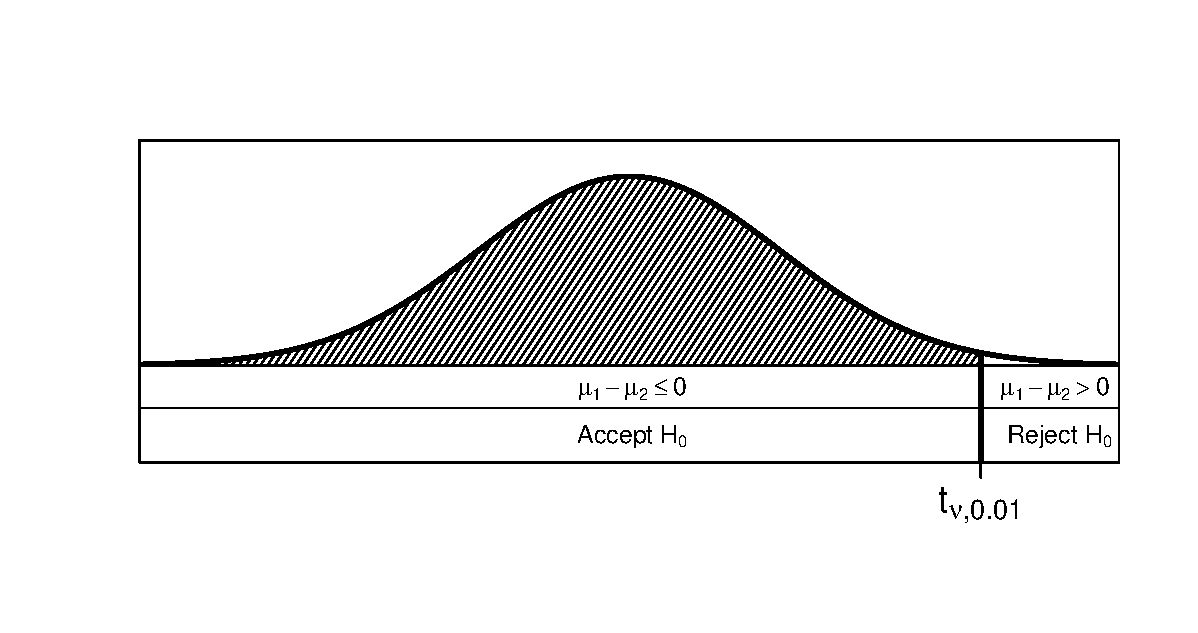
\includegraphics[width=0.8\textwidth, trim = 1.5cm 1.6cm 0.7cm 1.5cm, clip]{RejectRegion}
\end{center}

\end{frame}





\subsection{Example: CPU Temperature}
\begin{frame}{\bf \tcb{Example: CPU Temperature}}

The data was collected and the results are:
\begin{center}
\begin{tabular}{|c|c|c|}
\hline
&&\\[-0.3cm]
& Current & New \\
\hline
&&\\[-0.2cm]
sample size      & 6 & 4 \\[0.2cm]
mean   &  32.0\,$^\circ$C  & 29.2\,$^\circ$C \\[0.2cm]
standard deviation & 2.4\,$^\circ$C & 1.3\,$^\circ$C \\[0.2cm]
\hline
\multicolumn{2}{c}{}
\end{tabular}
\end{center}

Note that we have $s_1 = 2.4$ and $s_2 = 1.3$.\\[0.6cm]

For our calculations we will need:
\begin{align*}
s_1^2 &= (2.4)^2 = 5.76 &s_2^2 &= (1.3)^2 = 1.69
\end{align*}

\end{frame}





\subsection{Example: CPU Temperature (Equal Variances)}
\begin{frame}{\bf \tcb{Example: CPU Temperature (Equal Variances)}}

If we wish to assume {\bf equal variances} then we must first carry out the F-test to see that this assumption is reasonable.\\[0.4cm]

The null and alternative hypotheses for the F-test are:
\begin{align*}
H_0:\quad \sigma_1^2 &= \sigma_2^2 \\[0.2cm]
H_a:\quad \sigma_1^2 &\ne \sigma_2^2 \\[-0.4cm]
\end{align*}

The test statistic is $F = \frac{s_{\text{larger}}^2}{s_{\text{smaller}}^2} = \frac{5.76}{1.69} = 3.41$.\\[-0.1cm]
\begin{align*}\left.
\begin{array}{l}
\nu_1 = n_{\text{\,top}}-1 = 6-1=5 \\[0.3cm]
\nu_2 = n_{\text{\,bottom}}-1 = 4-1=3
\end{array}\right\} \Rightarrow F_{\,5,\,3}=14.9.\\[-0.4cm]
\end{align*}
{\footnotesize(Note: $F_{\,5,\,3}=14.9$ is the value in brackets from the F tables which corresponds to the 5\% level. For simplicity we will \emph{always} use the 5\% level for the F test.)}

\end{frame}




\subsection{Example: CPU Temperature (Equal Variances)}
\begin{frame}{\bf \tcb{Example: CPU Temperature (Equal Variances)}}

For the F-test, the rejection region is that \emph{above} the critical value.\\[0.4cm]

Since $F=3.41$ is below $14.9$, we accept $H_0:\, \sigma_1^2 = \sigma_2^2$. Hence, the equal variance assumption is reasonable.\\[0.8cm]

We will need the pooled variance:\\[-0.2cm]
\begin{align*}
s_p^2 = \frac{(n_1-1)\,s_1^2+(n_2-1)\,s_2^2}{n_1+n_2-2} &= \frac{(6-1)\,(5.76)+(4-1)\,(1.69)}{6+4-2} \\
&= \frac{33.87}{8} = 4.234.\\[-0.3cm]
\end{align*}
Also note that $\nu = n_1+n_2-2 = 6+4-2=8$.

\end{frame}




\subsection{Example: CPU Temperature (Equal Variances)}
\begin{frame}{\bf \tcb{Example: CPU Temperature (Equal Variances)}}
Recall that\\[-1.2cm]
\begin{align*}
H_0:\quad \mu_1-\mu_2 &\le 0 \\[0.2cm]
H_a:\quad \mu_1-\mu_2 &> 0 \\[-0.4cm]
\end{align*}
and we are testing at the $\alpha=0.01$ level $\Rightarrow$ $t_{\,8,\,0.01} = 2.896$ is the critical value (above which the rejection region lies).\\[0.4cm]
The test statistic is
\begin{align*}
t=\frac{(\bar x_1 - \bar x_2)-(\mu_{01}-\mu_{02})}{\sqrt{\frac{s_p^2}{n_1}+\frac{s_p^2}{n_2}}}=
\frac{(32.0 - 29.2)-(0)}{\sqrt{\frac{4.234}{6}+\frac{4.234}{4}}} = \frac{2.8}{1.3282} = 2.11.
\end{align*}
Since this is below $2.896$, we cannot reject $H_0$ at the 1\% level.\\[0.4cm]

Conclusion: we will continue to assume that the current CPU is superior to the new model (i.e., the current model runs cooler).

\end{frame}

%
%
%\subsection{Example: CPU Temperature (Equal Variances)}
%\begin{frame}{\bf \tcb{Example: CPU Temperature (Equal Variances)}}
%
%As this is a one-tailed test and $H_a$ contains the ``$>$'' sign, the p-value is calculated via $\Pr(Z>z)$ where $z$ is the test statistic.\\[0.8cm]
%
%However, since the samples are small, we have replaced $z$ with $t$.
%\begin{align*}
%\Rightarrow \text{p-value} = \Pr(T>t) = \Pr(T>2.11).\\[-0.3cm]
%\end{align*}
%
%We cannot find this value exactly from the t-tables. However, for $\nu=8$, we find $\Pr(T > 1.86) = 0.05$ and $\Pr(T > 2.306)=0.025$.\\[0.8cm]
%
%Thus, the p-value is between 0.025 and 0.05 $\Rightarrow$ there is evidence against $H_0$ but not enough to reject at the $\alpha=0.01$ level.\\[0.4cm]
%
%{\footnotesize(note: \texttt{R} calculates the p-value exactly when we run \texttt{t.test})}
%
%\end{frame}
%





\subsection{Example: CPU Temperature (Unequal Variances)}
\begin{frame}{\bf \tcb{Example: CPU Temperature (Unequal Variances)}}

For the {\bf unequal variance} approach we need to calculate:\\
\begin{align*}
a &= \frac{s_1^2}{n_1} = \frac{5.76}{6} = 0.96, &
b &= \frac{s_2^2}{n_2} = \frac{1.69}{4} = 0.4225.\\[-0.5cm]
\end{align*}
\begin{align*}
\Rightarrow \nu = \frac{(a+b)^2}{\frac{a\,^2}{n_1-1}+\frac{b\,^2}{n_2-1}} = \frac{(0.96+0.4225)^2}{\frac{0.96\,^2}{6-1}+\frac{0.4225\,^2}{4-1}}
= \frac{1.911}{0.2438} = 7.84.\\
\end{align*}
Since only whole number $\nu$ values appear in the tables, we round this to $\nu = 8$ $\Rightarrow$ the critical value is $t_{\,8,0.01} = 2.896$.

\end{frame}





\subsection{Example: CPU Temperature (Unequal Variances)}
\begin{frame}{\bf \tcb{Example: CPU Temperature (Unequal Variances)}}

The test statistic is\\[0.2cm]
\begin{align*}
t=\frac{(\bar x_1 - \bar x_2)-(\mu_{01}-\mu_{02})}{\sqrt{\frac{s_1^2}{n_1}+\frac{s_2^2}{n_2}}}=
\frac{(32.0 - 29.2)-(0)}{\sqrt{\frac{5.76}{6}+\frac{1.69}{4}}} = \frac{2.8}{1.1758} = 2.38.\\
\end{align*}
Since this is below $2.896$, we cannot reject $H_0$ at the 1\% level, i.e., the conclusion is the same as the equal variance approach here.\\[0.6cm]

%It is worth noting that the two approaches often do lead to similar results. However, the unequal variance approach doesn't require the \emph{assumption} that $\sigma_1^2=\sigma_2^2.$

\end{frame}




\section{Difference Between Two Proportions}
\subsection{Difference Between Two Proportions}
\begin{frame}{\bf \tcb{Difference Between Two Proportions}}

When comparing two proportions via hypothesis testing, the standard error for the difference is:\\[-0.1cm]
\begin{align*}
\boxed{s(\,\widehat{\!P}_1 - \,\widehat{\!P}_2) = \sqrt{\frac{\hat p_c \, (1-\hat p_c)}{n_1}+\frac{\hat p_c \, (1-\hat p_c)}{n_2}}\,}\,,\\[-0.1cm]
\end{align*}
where $\hat p_c$ is the {\bf combined proportion} over both groups:\\
\begin{align*}
\boxed{\hat p_c = \frac{x_1+x_2}{n_1+n_2}}.\\[-0.2cm]
\end{align*}

Thus, as was the case with one proportion, the standard error is different to that used in the case of a confidence interval.
\end{frame}


\subsection{Difference Between Two Proportions}
\begin{frame}{\bf \tcb{Difference Between Two Proportions}}

For testing the difference between two proportions we have:\\[0.3cm]

\begin{center}
\begin{tabular}{|c|c|c|c|}
\hline
&&&\\[-0.1cm]
Parameter & Statistic & Standard Error & Samples\\[0.3cm]
\hline
&&&\\[-0.1cm]
$p_1-p_2$ & $\hat p_1 - \hat p_2$  & ${\displaystyle\sqrt{\frac{\hat p_c\,(1-\hat p_c)}{n_1}+\frac{\hat p_c\,(1-\hat p_c)}{n_2}}}$ & large \\[0.8cm]
&&where\,\, ${\displaystyle \hat p_c = \frac{x_1+x_2}{n_1+n_2}}$&\\[-1.3cm]
&&& {\footnotesize(hypothesis test)}\\[1.1cm]
\hline
\multicolumn{4}{c}{}\\[0.5cm]
\end{tabular}
\end{center}



\end{frame}



\subsection{Example: Concept Design}
\begin{frame}{\bf \tcb{Example: Concept Design}}

A car manufacturer has developed a concept design. The company wish to test the hypothesis that there is no difference between the proportions of younger and older people who like the concept design using the 10\% level of significance.\\[0.8cm]

The null and alternative hypotheses are
\begin{align*}
H_0:\quad p_1 - p_2 &= 0\\[0.2cm]
H_a:\quad p_1 - p_2 &\ne 0\\[-0.3cm]
\end{align*}
With $\alpha=0.1$, and this being a two tailed test, the critical values are $\pm z_{0.05} = \pm 1.64$.

\end{frame}


\subsection{Example: Concept Design}
\begin{frame}{\bf \tcb{Example: Concept Design}}
The following data was collected:
\begin{center}
\begin{tabular}{|c|c|c|}
\hline
&&\\[-0.3cm]
& Younger & Older \\
\hline
&&\\[-0.2cm]
Sample size      & 158 & 91 \\[0.2cm]
Like concept   &  122  & 60 \\[0.2cm]
\hline
\multicolumn{2}{c}{}
\end{tabular}
\end{center}
Therefore
\begin{align*}
\hat p_1 &= \frac{122}{158} = 0.7722, & \hat p_2 &= \frac{60}{91} = 0.6593,
\end{align*}
and
\begin{align*}
\hat p_c &= \frac{122+60}{158+91} = \frac{182}{249} = 0.7309.
\end{align*}

\end{frame}


\subsection{Example: Concept Design}
\begin{frame}{\bf \tcb{Example: Concept Design}}

The test statistic is:\\[-0.1cm]
\begin{align*}
z= \frac{(\hat p_1 - \hat p_2) - (p_{01}-p_{02})}{\sqrt{\frac{\hat p_c\,(1-\hat p_c)}{n_1}+\frac{\hat p_c\,(1-\hat p_c)}{n_2}}} &= \frac{(0.7722 - 0.6593) - 0}{\sqrt{\frac{0.7309\,(0.2691)}{158}+\frac{0.7309\,(0.2691)}{91}}} \\[0.3cm]
&= \frac{0.1129}{0.0584} = 1.933.\\
\end{align*}

As this is outside of $\pm 1.64$, we reject the null hypothesis at the 10\% level $\Rightarrow$ we accept that the true proportions are different.\\[0.8cm]

Conclusion: The concept design is more appealing to younger people.

\end{frame}



\subsection{Example: Concept Design}
\begin{frame}{\bf \tcb{Example: Concept Design}}

We can also calculate a p-value. Being a two-tailed test, this is:\\
\begin{align*}
\text{p-value} = 2\times\Pr(Z>|1.933|) &= 2\times\Pr(Z>1.933) \\[0.2cm]
&= 2(0.0268) = 0.0536.\\[-0.2cm]
\end{align*}
The p-value is small and, hence, there is evidence against $H_0$.\\[0.8cm]

Clearly we can reject $H_0$ at the 10\% level of significance but it is worth noting that the evidence against $H_0$ is almost at the 5\% level.

\end{frame}


\section{R Code\hspace{1.5cm}}
\subsection{R Code: \texttt{t.test}}
\begin{frame}{\bf \tcb{R Code: \texttt{t.test}}}

The code for producing a confidence interval using \texttt{t.test} was given in Lecture14. You will notice that the output of the \texttt{t.test} function contains more than just a confidence interval.\\[0.8cm]

The function also displays the test statistic and corresponding p-value for a hypothesis test.\\[0.8cm]

The direction of the test is set using the $\boxed{\text{\texttt{alternative}}}$ option which must be one of  \texttt{"two.sided"} (the default),  \texttt{"less"} or \texttt{"greater"}.\\[0.8cm]

The hypothesised value is set using the $\boxed{\text{\texttt{mu}}}$ option (default is \texttt{mu=0}).\\[0.1cm]
{\footnotesize(note: \texttt{mu} represents the hypothesised mean in the case of one group and the hypothesised \emph{difference} in means in the case of two groups)}

\end{frame}


\subsection{R Code: One Mean}
\begin{frame}{\bf \tcb{R Code: One Mean}}

Consider the data from slide 14 of Lecture15 where we tested the hypothesis that the average CPU speed is 2.5Ghz. Thus:\\[-0.4cm]
\begin{align*}
H_0: \quad \mu &= 2.5\\[0.2cm]
H_a: \quad \mu &\ne 2.5\\[-0.5cm]
\end{align*}
We can test this hypothesis as follows:\\[0.3cm]
\begin{tabular}{|l|}
\hline
\texttt{cpu = c(2.53, 2.55, 2.54, 2.24)}\\[0.2cm]
\texttt{t.test(cpu, mu=2.5)}\\
\hline
\multicolumn{1}{c}{}\\[0.2cm]
\end{tabular}

Note: we do not have to specify \texttt{alternative} here since, by default this is already \texttt{alternative="two.sided"}.


\end{frame}



\subsection{R Code: One Mean}
\begin{frame}{\bf \tcb{R Code: One Mean}}

Output of\,\, \texttt{t.test(cpu, mu=2.5)}:\\[0.3cm]

\begin{footnotesize}
\begin{tabular}{|l|}
\hline
\texttt{One Sample t-test}\\[0.2cm]
\texttt{data:  cpu}\\
\texttt{t = -0.466, df = 3, p-value = 0.673}\\
\texttt{alternative hypothesis: true mean is not equal to 2.5}\\
\texttt{95 percent confidence interval:}\\
\texttt{ 2.225963 2.704037}\\
\texttt{sample estimates:}\\
\texttt{mean of x}\\
\texttt{    2.465 }\\
\hline
\multicolumn{1}{c}{}\\[0.0cm]
\end{tabular}
\end{footnotesize}
\begin{itemize}\itemsep0.2cm
\item \texttt{t = -0.466} is the test statistic.
\item \texttt{df = 3} is the degrees of freedom.
\item \texttt{p-value = 0.673} $\Rightarrow$ no evidence to reject $H_0: \, \mu = 2.5$.
\item Also note that the 95\% CI contains the value 2.5Ghz.
\end{itemize}


\end{frame}



\subsection{R Code: One Mean}
\begin{frame}{\bf \tcb{R Code: One Mean}}

If we wanted to assume that the average speed was 2.5Ghz or more then we would have:\\[-0.4cm]
\begin{align*}
H_0: \quad \mu &\ge 2.5\\[0.2cm]
H_a: \quad \mu &< 2.5\\[-0.2cm]
\end{align*}
We can test this hypothesis as follows:\\[0.4cm]
\begin{tabular}{|l|}
\hline
%\texttt{cpu = c(2.53, 2.55, 2.54, 2.24)}\\[0.2cm]
\texttt{t.test(cpu, alternative="less", mu=2.5)}\\
\hline
\multicolumn{1}{c}{}\\[0.2cm]
\end{tabular}

\end{frame}



\subsection{R Code: One Mean}
\begin{frame}{\bf \tcb{R Code: One Mean}}

Output of\,\, \texttt{t.test(cpu, alternative="less", mu=2.5)}:\\[0.3cm]

\begin{footnotesize}
\begin{tabular}{|l|}
\hline
\texttt{One Sample t-test}\\[0.2cm]
\texttt{data:  cpu}\\
\texttt{t = -0.466, df = 3, p-value = 0.3365}\\
\texttt{alternative hypothesis: true mean is less than 2.5}\\
\texttt{95 percent confidence interval:}\\
\texttt{ -Inf 2.641764}\\
%\texttt{sample estimates:}\\
%\texttt{mean of x}\\
%\texttt{    2.465 }\\
\hline
\multicolumn{1}{c}{}\\[0.0cm]
\end{tabular}
\end{footnotesize}
\begin{itemize}\itemsep0.3cm
\item Note that the test statistic and degrees of freedom are the same but the p-value has changed since this is a one-tailed test.
\item \texttt{p-value = 0.3365} $\Rightarrow$ no evidence to reject $H_0: \, \mu \ge 2.5$.
\item \texttt{R} also produces a one-tailed confidence interval - {\bf ignore this}.
\end{itemize}

\end{frame}



\subsection{R Code: Difference Between Means}
\begin{frame}{\bf \tcb{R Code: Difference Between Means}}
Consider the example on slide 18 of Lecture14. We wish to test the hypothesis that graduates from two universities have the same salary:
\begin{align*}
H_0: \quad \mu_1 - \mu_2 &= 0\\[0.2cm]
H_a: \quad \mu_1 - \mu_2 &\ne 0\\[-0.2cm]
\end{align*}

We can test this hypothesis as follows:\\[0.4cm]
\begin{tabular}{|l|}
\hline
\texttt{uni1 = c(32.1, 32.4, 33.2, 33.3, 33.6)}\\
\texttt{uni2 = c(35.7, 36.3, 39.4, 40.5)}\\
\texttt{t.test(uni1, uni2)}\\
\hline
\multicolumn{1}{c}{}\\[0.2cm]
\end{tabular}

We do not need to specify \texttt{alternative="two.sided"} or \texttt{mu=0} since these are the defaults.

\end{frame}




\subsection{R Code: Difference Between Means}
\begin{frame}{\bf \tcb{R Code: Difference Between Means}}

Output of\,\, \texttt{t.test(uni1, uni2)}:\\[0.3cm]

\begin{footnotesize}
\begin{tabular}{|l|}
\hline
\texttt{ Welch Two Sample t-test}\\[0.2cm]
\texttt{data:  uni1 and uni2}\\
\texttt{t = -4.2023, df = 3.359, p-value = 0.01961}\\
\texttt{alternative hypothesis:}\\
\texttt{true difference in means is not equal to 0}\\[0.1cm]
\texttt{95 percent confidence interval:}\\
\texttt{ -8.661686 -1.448314}\\
\texttt{sample estimates:}\\
\texttt{mean of x mean of y}\\
\texttt{   32.920    37.975}\\
\hline
\multicolumn{1}{c}{}\\[0.0cm]
\end{tabular}
\end{footnotesize}
\begin{itemize}\itemsep0.3cm
\item \texttt{p-val = 0.01961} $\Rightarrow$ strong evidence against $H_0:  \mu_1-\mu_2 = 0$.
\item We are not assuming equal variances here. In order to do so, use the option \texttt{var.equal=TRUE}.
\end{itemize}

\end{frame}




\subsection{R Code: Difference Between Means}
\begin{frame}{\bf \tcb{R Code: Difference Between Means}}
Consider the example from slide 12 of this lecture where we compared the temperatures of two CPU designs. In this case, it was assumed that the current CPU runs cooler and hence:
\begin{align*}
H_0: \quad \mu_1 - \mu_2 &\le 0\\[0.2cm]
H_a: \quad \mu_1 - \mu_2 &> 0\\[-0.5cm]
\end{align*}
We can test this hypothesis as follows:\\[0.2cm]
\begin{tabular}{|l|}
\hline
\texttt{cpu1 = c(33, 31, 32, 35, 33, 28)}\\
\texttt{cpu2 = c(29, 28, 29, 31)}\\
\texttt{t.test(cpu1, cpu2, alternative="greater")}\\[0.2cm]
\hline
\multicolumn{1}{c}{}\\[-0.2cm]
\end{tabular}

If we wish to assume equal variances then use:\\[0.2cm]
\begin{tabular}{|l|}
\hline
\texttt{t.test(cpu1, cpu2, alternative="greater",}\\
\hspace{5cm}\texttt{var.equal=TRUE)}\\
\hline
\multicolumn{1}{c}{}\\[0.2cm]
\end{tabular}

\end{frame}


\subsection{R Code: Difference Between Means}
\begin{frame}{\bf \tcb{R Code: Difference Between Means}}

Not assuming equal variances (compare with slide 19 of this lecture): \\[0.2cm]
\begin{tabular}{|l|}
\hline
\texttt{ Welch Two Sample t-test}\\[0.2cm]
\texttt{data:  cpu1 and cpu2}\\
\texttt{t = 2.3853, df = 7.802, p-value = 0.02247}\\
\texttt{alternative hypothesis:}\\
\texttt{true difference in means is greater than 0}\\
%95 percent confidence interval:
% 0.5990488       Inf
%sample estimates:
%mean of x mean of y
%    32.00     29.25
\hline
\multicolumn{1}{c}{}\\[-0.0cm]
\end{tabular}

Assuming equal variances (compare with slide 17 of this lecture):\\[0.2cm]
\begin{tabular}{|l|}
\hline
\texttt{ Two Sample t-test}\\[0.2cm]
\texttt{data:  cpu1 and cpu2}\\
\texttt{t = 2.1056, df = 8, p-value = 0.03417}\\
\texttt{alternative hypothesis:}\\
\texttt{true difference in means is greater than 0}\\
%95 percent confidence interval:
% 0.3213639       Inf
%sample estimates:
%mean of x mean of y
%    32.00     29.2
\hline
\multicolumn{1}{c}{}\\[0.2cm]
\end{tabular}

\end{frame}



\subsection{R Code: Ratio of Variances}
\begin{frame}{\bf \tcb{R Code: Ratio of Variances}}
The F-test investigates the ratio of two variances. The null and alternative hypotheses for this test are:\\[-0.2cm]
\begin{align*}
H_0: \quad \sigma^2_1 &= \sigma^2_2 \\[0.2cm]
H_a: \quad \sigma^2_1 &\ne \sigma^2_2\\[-0.3cm]
\end{align*}

For the CPU data we can carry out this test as follows:\\[0.3cm]
\begin{tabular}{|l|}
\hline
\texttt{var.test(cpu1, cpu2)}\\[0.2cm]
\hline
\multicolumn{1}{c}{}\\[-0.2cm]
\end{tabular}

\end{frame}




\subsection{R Code: Ratio of Variances}
\begin{frame}{\bf \tcb{R Code: Ratio of Variances}}

Output of\,\, \texttt{var.test(cpu1, cpu2)}:\\[-0.2cm]
\begin{adjustwidth}{-0.3cm}{0cm}
\begin{tabular}{|l|}
\hline
\texttt{ F test to compare two variances}\\[0.2cm]
\texttt{data:  cpu1 and cpu2}\\
\texttt{F = 3.5368, num df = 5,denom df = 3, p-value = 0.3274}\\
\texttt{alternative hypothesis:}\\
\texttt{true ratio of variances is not equal to 1}\\[0.2cm]
\texttt{95 percent confidence interval:}\\
\texttt{  0.237614 27.458590}\\
\hline
\multicolumn{1}{c}{}\\[0.0cm]
\end{tabular}
\end{adjustwidth}
\begin{itemize}\itemsep0.3cm
\item \texttt{p-val = 0.3274} $\Rightarrow$ no evidence to reject $H_0:  \sigma_1^2 = \sigma_2^2$.
\item The confidence interval is for the \emph{ratio} of the true variances. Note that the above interval supports a true ratio of 1, i.e., no difference in variances.
\end{itemize}

\end{frame}



\subsection{R Code: One Proportion}
\begin{frame}{\bf \tcb{R Code: One Proportion}}

For proportions, we use \texttt{prop.test}.\\[0.5cm]

Consider the example from slide 34 of Lecture15 where a company wished to test the hypothesis that 70\% of its users are teenagers:
\begin{align*}
H_0: \quad p &= 0.7\\[0.2cm]
H_a: \quad p &\ne 0.7\\[-0.5cm]
\end{align*}

The hypothesis test is carried out as follows:\\[0.3cm]
\begin{tabular}{|l|}
\hline
\texttt{x = 40}\\
\texttt{n = 75}\\[0.2cm]
\texttt{prop.test(x, n, p=0.7)}\\
\hline
\multicolumn{1}{c}{}\\[0.2cm]
\end{tabular}


\end{frame}



\subsection{R Code: One Proportion}
\begin{frame}{\bf \tcb{R Code: One Proportion}}

Output of\,\, \texttt{prop.test(x, n, p=0.7)}:\\[0.2cm]
\begin{tabular}{|l|}
\hline
\texttt{data:  x out of n, null probability 0.7}\\
\texttt{X-squared = 9.1429, df = 1, p-value = 0.002497}\\
\texttt{alternative hypothesis: true p is not equal to 0.7}\\
\texttt{95 percent confidence interval:}\\
\texttt{ 0.4151494 0.6480820}\\
\texttt{sample estimates:}\\
\texttt{        p}\\
\texttt{0.5333333}\\
\hline
\multicolumn{1}{c}{}\\[-0.1cm]
\end{tabular}
\begin{itemize}\itemsep0.4cm
\item \texttt{p-val = 0.002} $\Rightarrow$ strong evidence against $H_0:  p = 0.7$.
\item Note: \texttt{R} uses a different method for proportion tests to what we use in this course - so the results may differ slightly to what we do by hand.
\end{itemize}

\end{frame}



\subsection{R Code: One Proportion}
\begin{frame}{\bf \tcb{R Code: One Proportion}}

Consider the example from slide 36 of Lecture15 concerning the opinion of a new operating system. Recall we had:
\begin{align*}
H_0: \quad p &\le 0.5\\[0.2cm]
H_a: \quad p &> 0.5\\[-0.5cm]
\end{align*}

The hypothesis test is carried out as follows:\\[0.3cm]
\begin{tabular}{|l|}
\hline
\texttt{x = 38}\\
\texttt{n = 65}\\[0.2cm]
\texttt{prop.test(x, n, alternative="greater", p=0.5)}\\
\hline
\multicolumn{1}{c}{}\\[0.2cm]
\end{tabular}

Again the result will differ slightly from what we have done.

\end{frame}





\subsection{R Code: Two Proportions}
\begin{frame}{\bf \tcb{R Code: Two Proportions}}

For the concept car example on slide 22 of this lecture we had
\begin{align*}
H_0:\quad p_1 - p_2 &= 0\\[0.2cm]
H_a:\quad p_1 - p_2 &\ne 0\\[-0.3cm]
\end{align*}

\begin{tabular}{|l|}
\hline
\texttt{x = c(122,60)}\\
\texttt{n = c(158,91)}\\[0.2cm]
\texttt{prop.test(x, n)}\\
\hline
\multicolumn{1}{c}{}\\[0.2cm]
\end{tabular}


The result will differ slightly from what we have done.



\end{frame}












\end{document} 